\subsection{Разработка исполнителя}

Процесс вычисления выполняется над выражениями из узлов абстрактного синтаксического дерева.
Такой вид интерпретатора, который работает с AST называется <<tree walking interpreter>> или древовидный интерпретатор.
В таком интерпретаторе выполняется обход AST и выполнение соответствующих операций для каждого узла.

Последним этапом в процессе обработки исходного кода является его исполнение.
До этого шага все выражения языка представляют собой набор символов, токенов или ветви абстрактного синтаксического дерева без какого-либо семантического значения.
На данном этапе выражения языка приобретают смысл, то есть начинают интерпретироваться и действовать в соответствии с правилами и инструкциями языка.

Этап исполнения выполняется непосредственно после семантического анализа.
Если во время семантического анализа в обрабатываемом выражении не было обнаружено ошибок, выполняется переход к его вычислению.
Вычисление выражения выполняется в зависимости от его типа, например,
для инфиксного выражения применяется указанная в нем операция над левым и правым операндами и формируется результат в виде объекта соответствующего типа,
содержащего результат операции, а для условного выражения сначала вычисляется значение условия,
а затем в зависимости от его результата выполняется либо основная ветвь (при значении условия «true»), либо альтернативная (при значении условия «false»).

Только лишь вычислять значения выражений недостаточно.
Нужно также сохранять значения переменных для того, чтоб к ним можно было обратиться при обнаружении в выражениях.
Чтобы обеспечить эту возможность введем окружение – структуру данных, хранящую информацию о переменных и связанных с ними значениях на время выполнения программы.
Таким образом, при объявлении переменной, информация о ней будет записываться в окружение, а при необходимости получить значение этой переменой – ее значение будет считано из окружения.

В качестве примера работы алгоритма на рисунках~\ref{f:eval_int_infix_expr}~-~\ref{f:eval_string_infix_expr} приведены схемы алгоритма вычисления некоторых выражений.

\clearpage

\begin{figure}[!htp]
	\centering
	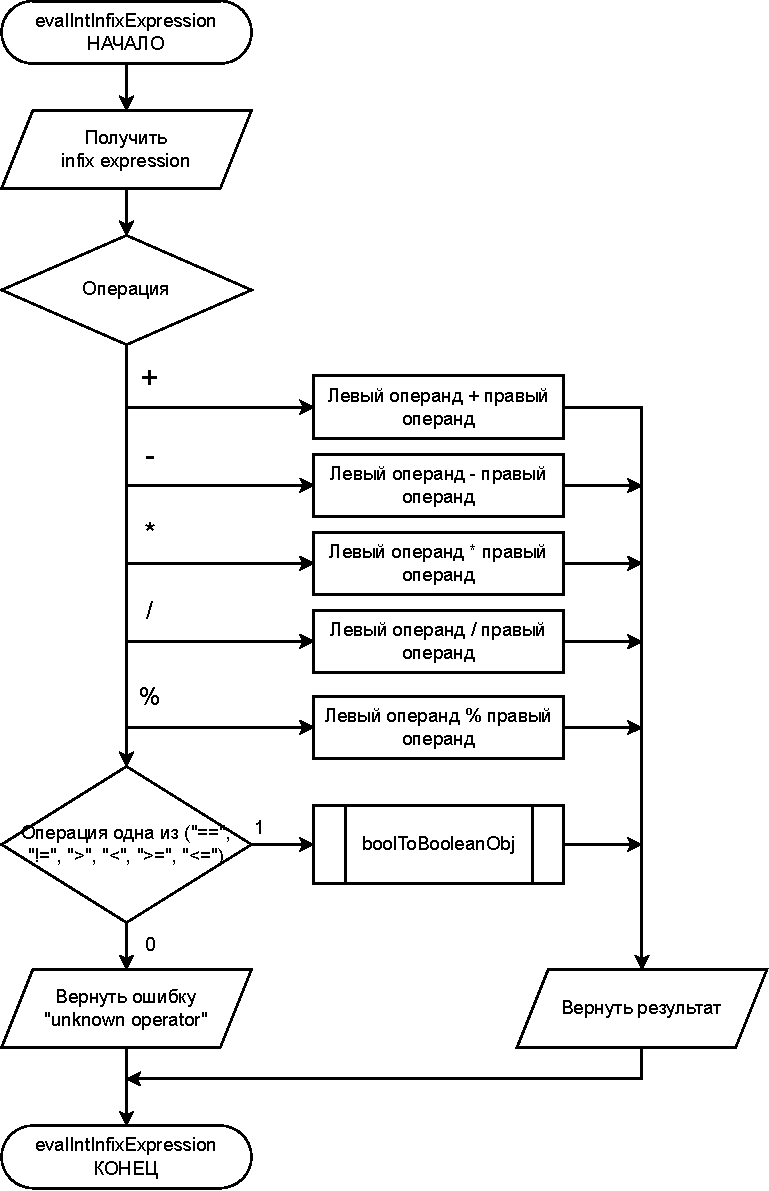
\includegraphics[width=0.8\textwidth]{structures/evaluator/eval_int_infix_expr.pdf}
	\caption{Схема алгоритма вычисления целочисленного инфиксного выражения}
	\label{f:eval_int_infix_expr}
\end{figure}

\clearpage

\begin{figure}[!htp]
	\centering
	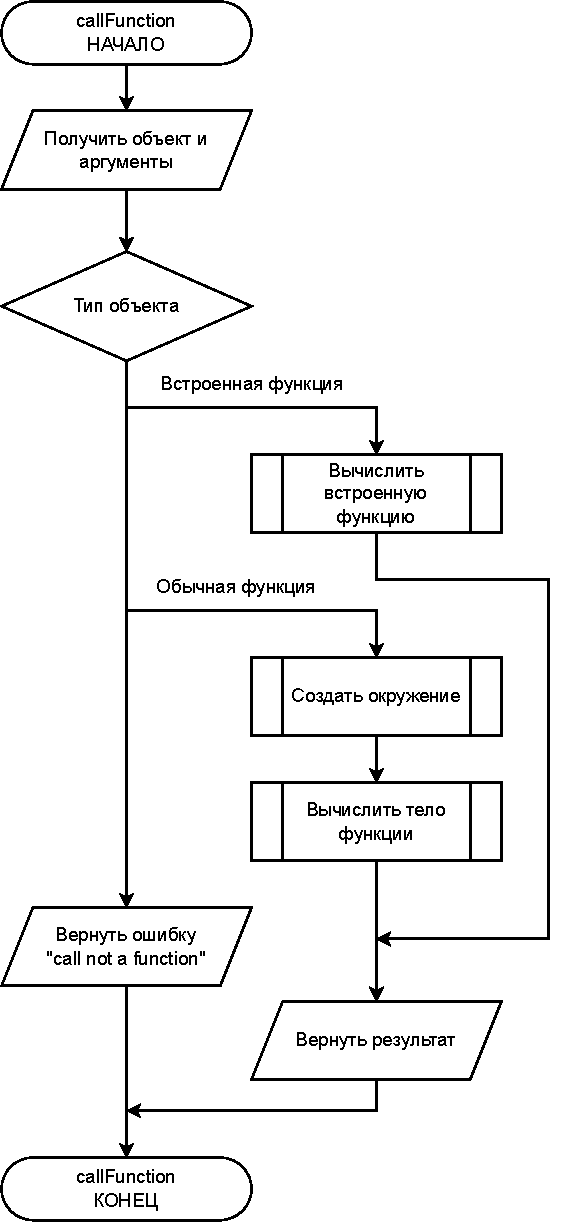
\includegraphics[width=0.6\textwidth]{structures/evaluator/eval_callFunction.pdf}
	\caption{Схема алгоритма исполнения вызова функции}
	\label{f:eval_callFunction}
\end{figure}

\clearpage

\begin{figure}[!htp]
	\centering
	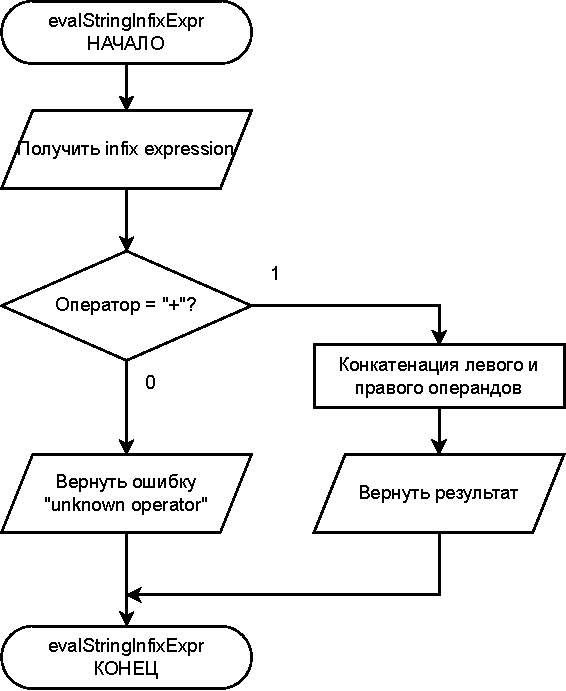
\includegraphics[width=0.5\textwidth]{structures/evaluator/eval_string_infix_expr.pdf}
	\caption{Схема алгоритма вычисления инфиксного выражения для строк}
	\label{f:eval_string_infix_expr}
\end{figure}